%!TEX program = xelatex
%!TEX TS-program = xelatex
%!TEX encoding = UTF-8 Unicode

\documentclass[a4paper, 12pt, centering]{article}



% ===========================页面设置===============================================
\usepackage{geometry}   %设置页边距的宏包
\geometry{left=2.5cm,right=2cm,top=2.5cm,bottom=2.5cm}  %设置 上、左、下、右 页边距

\usepackage{graphicx}  %插入图片的宏包
\usepackage{float} %设置图片浮动位置的宏包
\usepackage{subfigure} %插入多图时用子图显示的宏包
\usepackage[unicode]{hyperref} %超链接,支持unicode字符
\hypersetup{hidelinks} %隐藏超链接上的外框
\usepackage{xcolor}
\usepackage{indentfirst} %自动缩进

\usepackage{wallpaper} %background image
\addtolength{\wpYoffset}{8.0cm}
\usepackage{url}
\usepackage{fontspec,xltxtra,xunicode}
\defaultfontfeatures{Mapping=tex-text} %如果没有它,会有一些 tex 特殊字符无法正常使用,比如连字符
%文章内中文自动换行,可以自行调节
\XeTeXlinebreaklocale “zh”
\XeTeXlinebreakskip = 0pt plus 1pt minus 0.1pt

%%%% 下面的命令设置行间距与段落间距 %%%%
\linespread{1.4}
% \setlength{\parskip}{1ex}
\setlength{\parskip}{0.5\baselineskip}




% ===========================中文字体支持===============================================
% 字体需要根据自己电脑系统来设置
\usepackage{xeCJK}
\setmainfont{Times New Roman}
\setCJKmainfont{宋体}

\setCJKfamilyfont{zhhei}{黑体}
\newcommand*{\hei}{\CJKfamily{zhhei}}
\setCJKfamilyfont{zhkai}{楷体}
\newcommand*{\kai}{\CJKfamily{zhkai}}
\setCJKfamilyfont{enroman}{Times New Roman}
\newcommand*{\mytimes}{\CJKfamily{enroman}}




% ===========================数学符号===============================================
\usepackage{amsmath,amssymb}
\usepackage{bm} % $\bm{letter}$ 数学式中粗斜体字母的最佳方案
\usepackage{calc}
\usepackage{units} %单位宏包



% ===========================字号===============================================
\newcommand{\chuhao}{\fontsize{42pt}{\baselineskip}\selectfont}
\newcommand{\xiaochuhao}{\fontsize{36pt}{\baselineskip}\selectfont}
\newcommand{\yihao}{\fontsize{28pt}{\baselineskip}\selectfont}
\newcommand{\erhao}{\fontsize{21pt}{\baselineskip}\selectfont}
\newcommand{\xiaoerhao}{\fontsize{18pt}{\baselineskip}\selectfont}
\newcommand{\sanhao}{\fontsize{15.75pt}{\baselineskip}\selectfont}
\newcommand{\sihao}{\fontsize{14pt}{\baselineskip}\selectfont}
\newcommand{\xiaosihao}{\fontsize{12pt}{\baselineskip}\selectfont}
\newcommand{\wuhao}{\fontsize{10.5pt}{\baselineskip}\selectfont}
\newcommand{\xiaowuhao}{\fontsize{9pt}{\baselineskip}\selectfont}
\newcommand{\liuhao}{\fontsize{7.875pt}{\baselineskip}\selectfont}
\newcommand{\qihao}{\fontsize{5.25pt}{\baselineskip}\selectfont}



% ===========================定义摘要、关键词、章节等命令===============================================
\makeatletter
\renewcommand\abstract{%
\kai\textbf{\hei{摘要:}}
{\normalfont\xiaosihao\kai}}
\makeatother

\newenvironment{enabstract}

\makeatletter
\renewcommand\enabstract{%
\textbf{Abstract: }
{\normalfont\xiaosihao\mytimes}}
\makeatother

%%%% 设置 key words 属性 %%%%
\newenvironment{keys}

\makeatletter
\renewcommand\keys{%
\kai\textbf{\hei{关键词:}}
{\normalfont\xiaosihao\hei}}
\makeatother

\newenvironment{enkeys}

\makeatletter
\renewcommand\enkeys{%
\textbf{Key words: }
{\normalfont\xiaosihao\mytimes}}
\makeatother

%%%% 设置 section 属性 %%%%
\makeatletter
\renewcommand\section{\@startsection{section}{1}{\z@}%
{-1.5ex \@plus -.5ex \@minus -.2ex}%
{.5ex \@plus .1ex}%
{\normalfont\sihao\bf\hei}}
\makeatother

%%%% 设置 subsection 属性 %%%%
\makeatletter
\renewcommand\subsection{\@startsection{subsection}{1}{\z@}%
{-1.25ex \@plus -.5ex \@minus -.2ex}%
{.4ex \@plus .1ex}%
{\normalfont\xiaosihao\bf\hei}}
\makeatother

%%%% 设置 subsubsection 属性 %%%%
\makeatletter
\renewcommand\subsubsection{\@startsection{subsubsection}{1}{\z@}%
{-1ex \@plus -.5ex \@minus -.2ex}%
{.3ex \@plus .1ex}%
{\normalfont\xiaosihao\hei}}
\makeatother

%%%% 段落首行缩进两个字 %%%%
\makeatletter
\let\@afterindentfalse\@afterindenttrue
\@afterindenttrue
\makeatother
\setlength{\parindent}{2em}  %中文缩进两个汉字位






%%%% 定理类环境的定义 %%%%
\newtheorem{example}{例}             % 整体编号
\newtheorem{algorithm}{算法}
\newtheorem{theorem}{定理}[section]  % 按 section 编号
\newtheorem{definition}{定义}
\newtheorem{axiom}{公理}
\newtheorem{property}{性质}
\newtheorem{proposition}{命题}
\newtheorem{lemma}{引理}
\newtheorem{corollary}{推论}
\newtheorem{remark}{注解}
\newtheorem{condition}{条件}
\newtheorem{conclusion}{结论}
\newtheorem{assumption}{假设}

%%%% 重定义 %%%%
\renewcommand{\contentsname}{目录}  % 将Contents改为目录
\renewcommand{\abstractname}{摘要}  % 将Abstract改为摘要
\renewcommand{\refname}{参考文献}   % 将References改为参考文献
\renewcommand{\indexname}{索引}
\renewcommand{\figurename}{图}
\renewcommand{\tablename}{表}
\renewcommand{\appendixname}{附录}
\renewcommand{\algorithm}{算法}


%%%% 定义标题格式,包括title,author,affiliation,email等 %%%%
\title{\yihao{这里是大标题啊}}
\author{\xiaoerhao{作者姓名}\footnote{电子邮件: ***@***.com,学号: ***}\\[2ex]
\sanhao 东南大学网络空间安全学院\\[2ex]
}
\date{\sanhao\today}




% ===========================正正正正正正正==============================================
% ===========================文文文文文文文===============================================
% ===========================这这这这这这这===============================================
% ===========================里里里里里里里===============================================
% ===========================开开开开开开开===============================================
% ===========================始始始始始始始===============================================
% ===========================写写写写写写写===============================================
% ===========================哟哟哟哟哟哟哟===============================================



\begin{document}

%封面背景图片
%可以换其它自己想放的图片
\ThisCenterWallPaper{1.0}{seu.png}






%%%% 以下部分是正文 %%%%

%标题上方空出一些距离
\
\vspace{10cm}
\begingroup
\let\newpage\relax% Void the actions of \newpage
\maketitle
\endgroup
\newpage
%----------


%%% 摘要 %%%

\begin{abstract}
这里是摘要这里是摘要这里是摘要这里是摘要这里是摘要这里是摘要这里是摘要这里是摘要这里是摘要这里是摘要这里是摘要这里是摘要这里是摘要这里是摘要这里是摘要这里是摘要这里是摘要这里是摘要这里是摘要这里是摘要这里是摘要这里是摘要这里是摘要这里是摘要这里是摘要这里是摘要这里是摘要这里是摘要这里是摘要这里是摘要这里是摘要这里是摘要这里是摘要这里是摘要这里是摘要这里是摘要这里是摘要这里是摘要这里是摘要这里是摘要这里是摘要这里是摘要这里是摘要这里是摘要
\end{abstract}

\begin{keys}
关键词1;关键词2;关键词3
\end{keys}

\begin{enabstract}
Here is English abstract. Here is English abstract. Here is English abstract. Here is English abstract. Here is English abstract. Here is English abstract. Here is English abstract. Here is English abstract. Here is English abstract. Here is English abstract. Here is English abstract. Here is English abstract. Here is English abstract. Here is English abstract. Here is English abstract. Here is English abstract. Here is English abstract. Here is English abstract. Here is English abstract. Here is English abstract.
\end{enabstract}

\begin{enkeys}
keyword1, keyword2, keyword3
\end{enkeys}
\newpage

%%% 目录 %%%
\tableofcontents
\newpage

\section{第一节}
吴恩达1976年出生于伦敦,父亲是一位香港医生,英文名叫Andrew Ng,吴恩达年轻时候在香港和新加坡度过。

\subsection{第一节第一小节}
1992年吴恩达就读新加坡莱佛士书院,并于1997年获得了卡内基梅隆大学的计算机科学学士学位。之后他在1998年获得了麻省理工学院的硕士学位,并于2002年获得了加州大学伯克利分校的博士学位,并从这年开始在斯坦福大学工作。他(2002年)住在加利福尼亚州的帕洛阿尔托。

\subsubsection{第一节第一小节第一小小节}

吴恩达是斯坦福大学计算机科学系和电子工程系副教授,人工智能实验室主任。吴恩达主要成就在机器学习和人工智能领域,他是人工智能和机器学习领域最权威的学者之一。

\subsection{第一节第一小节第二小小节}
2010年,时任斯坦福大学教授的吴恩达加入谷歌开发团队XLab——这个团队已先后为谷歌开发无人驾驶汽车和谷歌眼镜两个知名项目。吴恩达与谷歌顶级工程师开始合作建立全球最大的“神经网络”,这个神经网络能以与人类大脑学习新事物相同的方式来学习现实生活。谷歌将这个项目命名为“谷歌大脑”。

\section{第二节}
\subsection{第二节第二小小节}
吴恩达最知名的是,所开发的人工神经网络通过观看一周YouTube视频,自主学会识别哪些是关于猫的视频。这个案例为人工智能领域翻开崭新一页。吴恩达表示,未来将会在谷歌无人驾驶汽车上使用该项技术,来识别车前面的动物或者小孩,从而及时躲避。2014年5月16日,百度宣布吴恩达加入百度,担任百度公司首席科学家,负责百度研究院的领导工作,尤其是Baidu Brain计划。2014年5月19日,百度宣布任命吴恩达博士为百度首席科学家,全面负责百度研究院。这是中国互联网公司迄今为止引进的最重量级人物。消息一经公布,就成为国际科技界的关注话题。美国权威杂志《麻省理工科技评论》(MIT Technology Review)甚至用充满激情的笔调对未来给予展望:“百度将领导一个创新的软件技术时代,更加了解世界。”

\subsection{引用}
文献\cite{1}\cite{2}叙述了。。。

\subsection{图片}
图\ref{Fig.main}如下所示:
\begin{figure}[H] %H为当前位置,!htb为忽略美学标准,htbp为浮动图形
\centering %图片居中
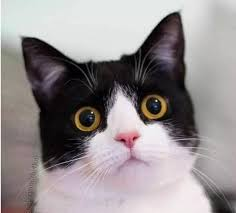
\includegraphics[width=0.8\textwidth]{example1.jpeg} %插入图片,[]中设置图片大小,{}中是图片文件名
\caption{Main name} %最终文档中希望显示的图片标题
\label{Fig.main} %用于文内引用的标签
\end{figure}

表\ref{tab.main}如下所示:
\begin{table}[H]
\centering
\caption{Test Caption.}
\begin{tabular}{|c|c|c|}
\hline
\multicolumn{3}{|c|}{学生信息}\\
\hline
姓名& 学号& 性别\\
\hline
Ch'en Meng& 001& Male\\
Sarah Brightman& 002& Female\\
\hline
\end{tabular}
\label{tab.main}
\end{table}


图\ref{Fig.sub.1},图\ref{Fig.sub.2},图\ref{Fig.sub.3}如下所示:
\begin{figure}[H]
\centering  %图片全局居中
\subfigure[name1]{
\label{Fig.sub.1}
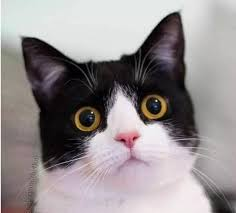
\includegraphics[width=0.3\textwidth]{example1.jpeg}}
\subfigure[name2]{
\label{Fig.sub.2}
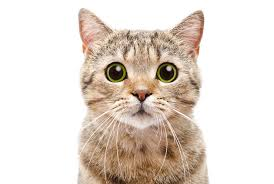
\includegraphics[width=0.3\textwidth]{example2.jpeg}}
\subfigure[name3]{
\label{Fig.sub.3}
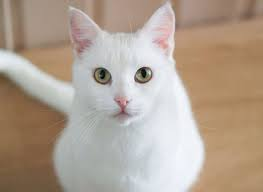
\includegraphics[width=0.3\textwidth]{example3.jpeg}}
\caption{Main name}
\label{Fig.main}
\end{figure}




\begin{thebibliography}{1}
\bibitem{1} Wray J, Green G G R. Neural networks, approximation theory, and finite precision computation[J]. Neural networks, 1995, 8(1): 31-37.
\bibitem{2} Ham F M, Kostanic I. Principles of neurocomputing for science and engineering[M]. McGraw-Hill Higher Education, 2000.
\end{thebibliography}

\end{document}
